\documentclass[aspectratio=169]{beamer}
\usepackage[utf8]{inputenc}
\usepackage[T1]{fontenc}
\usepackage[french]{babel}
\usepackage{graphicx}
\usepackage{pgfpages}
\usepackage{prftree}
\usepackage{tikz}
\usetikzlibrary{arrows.meta, positioning, decorations.pathreplacing, calc}
\usepackage[backend=biber, style=alphabetic, url=true]{biblatex}
\addbibresource{../../biblio.bib}

\graphicspath{{images/}}
\usetheme{Boadilla}
% \setbeameroption{show notes on second screen=right}

\title{Leçon 4 : Proof-theoretic semantics, vérificationnisme et pragmatisme}
\subtitle{Justification et encodage des règles logiques et calculatoires}
\author{Pablo Donato}
\institute{Logique et Fondements de l'Informatique}
\date{Année 2026}

\begin{document}

% ─────────────────────────────────────────────────────────────
% FRAME 1 — TITRE
% ─────────────────────────────────────────────────────────────
\begin{frame}
  \titlepage
  \note{
    Bonjour à tous. Rappel de la semaine dernière : on a utilisé la tactique \texttt{rewrite}
    sans vraiment l'expliquer. Je vous avais promis qu'on en comprendrait l'origine aujourd'hui.
    C'est l'occasion de poser une question philosophique plus profonde : qu'est-ce que cela signifie
    de \emph{définir} un connecteur logique ? Quelle règle lui donne son sens ?
  }
\end{frame}

% ─────────────────────────────────────────────────────────────
% FRAME 2 — LA QUESTION CENTRALE
% ─────────────────────────────────────────────────────────────
\begin{frame}{La question centrale : d'où vient le sens d'un connecteur ?}
  \pause
  En déduction naturelle, chaque connecteur possède deux types de règles :
  \begin{columns}
    \begin{column}{0.48\textwidth}
      \begin{center}
        \textbf{Introductions} — comment construire
        \medskip

        $\prftree[r]{${\vee}I_1$}{\Gamma \vdash A}{\Gamma \vdash A \vee B}$
        \quad
        $\prftree[r]{${\vee}I_2$}{\Gamma \vdash B}{\Gamma \vdash A \vee B}$
      \end{center}
    \end{column}
    \begin{column}{0.48\textwidth}
      \begin{center}
        \textbf{Élimination} — comment utiliser
        \medskip

        $\prftree[r]{${\vee}E$}
        {\Gamma \vdash A \vee B}
        {\Gamma, A \vdash C}
        {\Gamma, B \vdash C}
        {\Gamma \vdash C}$
      \end{center}
    \end{column}
  \end{columns}
  \bigskip
  \begin{alertblock}{Question philosophique}
    Lesquelles des deux sont \emph{premières} ? Lesquelles \textbf{définissent} ce que \emph{signifie} le connecteur ?
  \end{alertblock}
  \pause
  \begin{center}
    Deux grandes réponses en \emph{proof-theoretic semantics} (théorie de la démonstration).
  \end{center}
  \note{
    Poser la question rhétoriquement aux étudiants. Leur laisser 30 secondes.
    Les deux réponses sont philosophiquement défendables — c'est l'objet du débat
    qui opposera Prawitz/Dummett d'un côté à Dummett/Zeilberger de l'autre.
  }
\end{frame}

% ─────────────────────────────────────────────────────────────
% FRAME 3 — LE VÉRIFICATIONNISME
% ─────────────────────────────────────────────────────────────
\begin{frame}{Le vérificationnisme (Gentzen, Prawitz, Dummett)}
  \begin{block}{Principe}
    Le sens d'un connecteur = ses \textbf{conditions de vérification} = ses règles d'\textbf{introduction}.
  \end{block}
  \begin{itemize}
    \item Pour $\vee$ : prouver $A \vee B$, c'est apporter une preuve de $A$, ou une preuve de $B$.
      \pause
    \item Les règles d'élimination sont \textbf{dérivées canoniquement} \\
      (principe d'inversion de Prawitz) : une élimination est justifiée si elle
      \emph{préserve la canonicité des preuves}.
      \pause
    \item \textbf{Fundamental Assumption} (Dummett) : toute proposition prouvable possède
      une \emph{preuve canonique}, se terminant \emph{héréditairement} par une règle d'introduction.
      \begin{itemize}
        \item C'est un \emph{(meta-)théorème} en logique intuitionniste (normalisation de Prawitz).
        \item Il permet de remplacer la sémantique tarskiste par une sémantique de preuves.
        \item Philosophiquement : anti-réalisme, signification fondée sur l'usage \\
          (Wittgenstein) plutôt que sur la dénotation (Frege).
      \end{itemize}
  \end{itemize}
  \medskip
  \textit{Slogan : « On comprend $\vee$ parce qu'on sait comment le construire. »}
  \note{
    Insister sur l'enjeu philosophique : ce n'est pas un simple choix technique.
    La Fundamental Assumption est la clé : si toute preuve peut être normalisée (ramenée en
    forme canonique), alors définir la signification via les introducteurs est cohérent —
    on ne perd aucune information. C'est pour ça que le vérificationnisme est
    philosophiquement \emph{défendable}. Mentionner le lien avec le théorème de
    normalisation de Prawitz (1965) et le théorème d'élimination des coupures de Gentzen.
  }
\end{frame}

% ─────────────────────────────────────────────────────────────
% FRAME 4 — LE PRAGMATISME
% ─────────────────────────────────────────────────────────────
\begin{frame}{Le pragmatisme (Zeilberger §2.1, d'après Dummett)}
  \begin{block}{Principe}
    Le sens d'un connecteur = ses \textbf{conditions d'utilisation} = ses règles d'\textbf{élimination}.
  \end{block}
  \begin{itemize}
    \item (Dummett) : les éliminations sont tout aussi valides comme point de départ.
      \pause
    \item Pour $\vee$ : une preuve de $A \vee B$, c'est ce qui sait répondre à
      \emph{tout usage canonique} — i.e., produire $C$ dès qu'on sait dériver
      $C$ de $A$ et $C$ de $B$.
      \pause
    \item \textbf{Procédure de justification descendante} (duale de Prawitz) :
      une règle est valide si toute \emph{conséquence canoniquement obtenue}
      de sa conclusion peut être transformée en une conséquence canoniquement
      obtenue de ses prémisses.
      \begin{itemize}
        \item[$\uparrow$] Vérif. : preuve canonique = preuve \emph{terminant par} des introductions
        \item[$\downarrow$] Pragma. : conséquence canonique = conséquence \emph{commençant par} des éliminations
      \end{itemize}
  \end{itemize}
  \medskip
  \textit{Slogan : « On comprend $\vee$ parce qu'on sait à quoi il sert. »}
  \note{
    Les deux procédures de justification seront expliquées au tableau.
    L'idée clé : la procédure descendante est le miroir exact de la procédure
    ascendante de Prawitz. Là où Prawitz demande qu'une élimination préserve
    les preuves canoniques (normalisation), Dummett/Zeilberger demandent
    qu'une introduction préserve les conséquences canoniques.
    La notion de « conséquence canoniquement obtenue » = conséquence obtenue
    par une suite d'éliminations (l'analogue dual de la preuve canonique).
    Insister : c'est Dummett qui a mis en évidence la cohérence de cette approche.
  }
\end{frame}

% ─────────────────────────────────────────────────────────────
% FRAME 5 — LES TYPES INDUCTIFS : LE CHOIX DE ROCQ
% ─────────────────────────────────────────────────────────────
\begin{frame}[fragile]{Les types inductifs : le choix vérificationniste de Rocq}
  Rocq choisit le vérificationnisme : on \textbf{déclare les constructeurs} directement.
  \medskip

  Définitions réelles de la bibliothèque standard :
  \medskip
  \begin{columns}
    \begin{column}{0.48\textwidth}
\begin{verbatim}
Inductive and (A B : Prop) : Prop :=
  | conj : A -> B -> A /\ B.
\end{verbatim}
    \end{column}
    \begin{column}{0.48\textwidth}
\begin{verbatim}
Inductive or (A B : Prop) : Prop :=
  | or_introl : A -> A \/ B
  | or_intror : B -> A \/ B.
\end{verbatim}
    \end{column}
  \end{columns}
  \medskip
  \begin{itemize}
      \pause
    \item Les éliminateurs (\texttt{and\_ind}, \texttt{or\_ind})
      sont \textbf{dérivés automatiquement} — avec leur contenu calculatoire complet.
      \pause
    \item C'est le vérificationnisme incarné : les introductions définissent tout,
      les éliminations \emph{s'en suivent}.
  \end{itemize}
  \note{
    \texttt{conj}, \texttt{or\_introl}, \texttt{or\_intror} — ce sont exactement
    les constructeurs qu'ils utilisent depuis la Leçon 2 avec \texttt{split},
    \texttt{left}, \texttt{right}. Et \texttt{destruct} n'est rien d'autre que
    l'éliminateur automatiquement dérivé. On lève le voile sur la magie.
  }
\end{frame}

% ─────────────────────────────────────────────────────────────
% FRAME 6 — INTERLUDE : ENCODAGES CHURCH
% ─────────────────────────────────────────────────────────────
\begin{frame}{Interlude : encodages de Church des connecteurs}
  \begin{center}
    \begin{tabular}{ll}
      \hline
      \textbf{Connecteur} & \textbf{Encodage de Church (pragmatiste)} \\
      \hline
      $A \vee B$ & $\forall P,\; (A \to P) \to (B \to P) \to P$ \\[4pt]
      $A \wedge B$ & $\forall P,\; (A \to B \to P) \to P$ \\[4pt]
      $\bot$ & $\forall P,\; P$ \\[4pt]
      $\exists x,\; P\,x$ & $\forall Q,\; (\forall x,\; P\,x \to Q) \to Q$ \\
      \hline
    \end{tabular}
  \end{center}
  \medskip
  \begin{itemize}
    \item Valides dans le \textbf{Calcul des Constructions pur} (sans \texttt{Inductive}).
    \item En logique du 2\textsuperscript{nd} ordre — ce qui est le cas de Rocq, où l'on
      peut quantifier sur \texttt{Prop}.
    \item Logiquement correctes, mais \emph{coûteuses en pratique}.
  \end{itemize}
  \note{
    $\bot$ encodé dit « tout ce qu'on veut pour n'importe quelle conclusion » —
    c'est la règle \emph{ex falso quodlibet} incarnée directement dans le type.
    L'existentiel Church dit « je suis ce qui sait répondre à n'importe quelle
    continuation qui consomme un témoin ».
    Faire remarquer que l'encodage de $A \wedge B$ lit : « pour toute conclusion $P$,
    si tu sais produire $P$ à partir de $A$ et $B$ ensemble, alors je te donne $P$ »
    — c'est l'éliminateur de la conjonction.
  }
\end{frame}

% ─────────────────────────────────────────────────────────────
% FRAME 7 — POURQUOI ROCQ CHOISIT INDUCTIVE
% ─────────────────────────────────────────────────────────────
\begin{frame}{Pourquoi Rocq choisit \texttt{Inductive} plutôt que Church}
  Les deux approches sont \textbf{logiquement équivalentes} en logique du 2\textsuperscript{nd}
  ordre (Rocq peut quantifier sur \texttt{Prop}).

  \medskip
  Mais l'encodage de Church a des coûts calculatoires sérieux :
  \begin{itemize}
    \item Une preuve de $A \vee B$ est une \emph{fonction} ($\lambda$-terme), pas une donnée :
      son usage nécessite des $\beta$-réductions coûteuses.
    \item Les structures de données encodées à la Church (listes, arbres…) sont
      inutilisables pour de vrais programmes car trop lentes (complexité en temps).
  \end{itemize}
  \pause
  Avec \texttt{Inductive} :
  \begin{itemize}
    \item Représentation \textbf{concrète en mémoire} (e.g. les paires et injections vues
      en Leçon 2).
    \item \textbf{Pattern-matching} compilable directement en code machine efficace.
    \item Éliminateurs dérivés avec leur contenu calculatoire complet.
  \end{itemize}
  \pause
  \begin{alertblock}{L'ironie}
    Rocq choisit le vérificationnisme pour des raisons\ldots{} \emph{pragmatiques} !
  \end{alertblock}
  \note{
    L'ironie est à savourer. La question philosophique a des conséquences techniques
    profondes. Les encodages Church sont magnifiques théoriquement, mais impraticables
    pour une vérification à grande échelle.
  }
\end{frame}

% ─────────────────────────────────────────────────────────────
% FRAME 8 — L'ÉGALITÉ REVISITÉE
% ─────────────────────────────────────────────────────────────
\begin{frame}[fragile]{L'égalité revisitée : \texttt{eq} est inductive}
  La définition réelle de \texttt{=} dans Rocq :
  \medskip
\begin{verbatim}
  Inductive eq (A : Type) (x : A) : A -> Prop :=
    | eq_refl : eq A x x.
\end{verbatim}
  \medskip
  \begin{itemize}
    \item Un \textbf{seul constructeur} : on ne peut prouver \texttt{x = y} qu'en
      exhibant que \texttt{x} et \texttt{y} sont \emph{le même objet}.
      \pause
    \item Définition vérificationniste \emph{maximalement restrictive} : la seule
      preuve canonique de \texttt{x = y} est la réflexivité.
      \pause
    \item L'éliminateur dérivé automatiquement est\ldots{} le \textbf{principe de Leibniz} :
      \begin{center}
        \fbox{$x = y$ \textit{ssi} pour toute propriété $P$,\; $P(x) \Rightarrow P(y)$}
      \end{center}
  \end{itemize}
  \note{
    Moment « aha ». On a utilisé \texttt{rewrite} comme une boîte noire la semaine
    dernière. Aujourd'hui on voit que c'est exactement l'éliminateur canonique
    (au sens de Prawitz !) du type inductif \texttt{eq}. Le vérificationnisme
    \emph{explique} et \emph{justifie} \texttt{rewrite}.
  }
\end{frame}

% ─────────────────────────────────────────────────────────────
% FRAME 9 — LEIBNIZ JUSTIFIÉ PAR PRAWITZ
% ─────────────────────────────────────────────────────────────
\begin{frame}{Leibniz justifié par Prawitz}
  \begin{columns}
    \begin{column}{0.65\textwidth}
      \textbf{Leibniz} (\emph{Discours de métaphysique}, 1686) :
      \begin{quote}
        Deux choses sont identiques si et seulement si elles partagent
        toutes leurs propriétés (\emph{indiscernabilité des identiques}).
      \end{quote}
      \pause
      \medskip
      Dans Rocq, \texttt{rewrite} = application de l'éliminateur de \texttt{eq}.
      \pause
      \\
      \textbf{La chaîne de justification :}
      \begin{enumerate}
        \item \texttt{eq} est défini avec un seul introducteur : \texttt{eq\_refl}
        \item Son éliminateur (dérivé vérificationnistiquement) = substitution universelle
        \item Cette substitution \emph{est} le principe de Leibniz
      \end{enumerate}
    \end{column}
    \begin{column}{0.3\textwidth}
      \begin{center}
        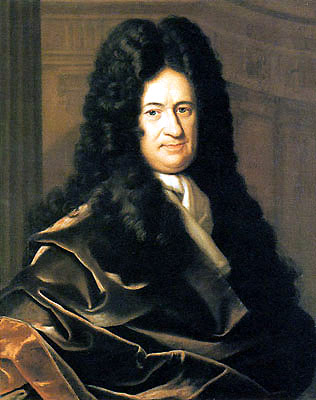
\includegraphics[width=0.85\textwidth]{leibniz.jpg}
      \end{center}
    \end{column}
  \end{columns}
  \note{
    C'est un des moments les plus satisfaisants philosophiquement. Une notion
    métaphysique classique (identité des indiscernables) se retrouve
    \emph{calculatoirement justifiée} par un principe de théorie de la démonstration.
    On ne « fait pas confiance » à la machine — on comprend \emph{pourquoi} elle
    fait ce qu'elle fait. Le vérificationnisme de Prawitz \emph{fonde} l'identité
    de Leibniz.
  }
\end{frame}

% ─────────────────────────────────────────────────────────────
% FRAME 10 — OUVERTURE : HoTT
% ─────────────────────────────────────────────────────────────
\begin{frame}{Ouverture : HoTT et au-delà de Leibniz}
  Que \emph{signifie} une preuve de \texttt{x = y} au-delà de la réflexivité ?
  \pause

  \begin{block}{Homotopy Type Theory — HoTT (Voevodsky, $\sim$2006--2013)}
    \begin{itemize}
      \item Interpréter les \emph{types} comme des \textbf{espaces topologiques}
        (au sens de la théorie de l'homotopie).
      \item Les \emph{termes} = points dans l'espace.
      \item Les \emph{preuves d'égalité} = \textbf{chemins} entre deux points.
      \item Une preuve de \texttt{x = y} peut avoir une \emph{structure propre} :
        plusieurs chemins distincts entre les mêmes points.
      \item \textbf{Axiome d'univalence} : deux types équivalents sont \emph{égaux}.
    \end{itemize}
  \end{block}

  \medskip
  La question « qu'est-ce que l'égalité ? » reste ouverte et philosophiquement/mathématiquement féconde.
  \note{
    Slide courte, pas de code. L'objectif est d'ouvrir une porte. Voevodsky
    (Médaille Fields 2010) a formalisé toute cette théorie dans un assistant de preuve
    (Agda/Coq). L'axiome d'univalence dit intuitivement que deux types qui se
    comportent de la même façon \emph{sont} le même type — ce que la réflexivité
    seule de \texttt{eq} ne capture pas. C'est un domaine de recherche actif
    aux frontières des mathématiques et de la philosophie.
  }
\end{frame}

% ─────────────────────────────────────────────────────────────
% FRAME 11 — OUVERTURE : CALCULUS OF UNITY (ZEILBERGER)
% ─────────────────────────────────────────────────────────────
\begin{frame}{Ouverture : le Calculus of Unity (Zeilberger, 2008)}
  Dummett a montré que les deux approches sont cohérentes. Zeilberger propose de les
  \textbf{unifier} en distinguant quatre jugements, sur le modèle du \emph{carré logique d'Aristote} :

  \medskip
  \begin{center}
    \begin{tikzpicture}[
        >=Stealth,
        box/.style={draw, rounded corners=4pt, text width=3.4cm, align=center,
        minimum height=1.1cm, font=\small},
        arr/.style={->, thick},
        darr/.style={<->, thick, dashed, gray},
        lbl/.style={font=\scriptsize, text=gray}
      ]
      % Nodes
      \node[box, fill=blue!10] (TL) at (0, 0)
      {\textbf{preuve directe} de $A$};
      \node[box, fill=blue!10] (TR) at (5.5, 0)
      {\textbf{réfutation justifiée} de $A$};
      \node[box, fill=orange!10] (BL) at (0, -3)
      {\textbf{preuve justifiée} de $A$};
      \node[box, fill=orange!10] (BR) at (5.5, -3)
      {\textbf{réfutation directe} de $A$};

      % Horizontal arrows (negation)
      \draw[arr] (TR) -- node[above, lbl] {négation} (TL);
      \draw[arr] (BL) -- node[below, lbl] {négation} (BR);

      % Vertical arrows (shifts)
      \draw[arr] (BL) -- node[left, lbl] {$\downarrow$ (shift)} (TL);
      \draw[arr] (TR) -- node[right, lbl] {$\uparrow$ (shift)} (BR);

      % Diagonal arrows (dualisation linéaire)
      \draw[darr] (TL) -- (BR);
      \draw[darr] (TR) -- node[above, lbl] {$(\cdot)^\bot$} (BL);

      % Half-labels
      \node[font=\scriptsize\bfseries, text=blue!70] at (2.75, 0.75)
      {sémantique vérificationniste (positif)};
      \node[font=\scriptsize\bfseries, text=orange!80!black] at (2.75, -3.75)
      {sémantique pragmatiste (négatif)};
    \end{tikzpicture}
  \end{center}

  Via Curry-Howard : \textbf{stratégies d'évaluation} (call-by-value ($+$) vs. call-by-name ($-$))

  \note{
    L'idée centrale de Zeilberger : les deux approches ne se contredisent pas —
    elles parlent de \emph{types de propositions} différents. Les propositions positives
    sont définies par leurs introductions (constructeurs), les négatives par leurs
    éliminations (continuations). La coupure entre une preuve positive et une réfutation
    produit une \emph{computation}. Lien avec call-by-value (positif) et call-by-name
    (négatif). Ne pas entrer dans les détails techniques. Les « shift connectives »
    (↑↓) font le pont entre les deux moitiés du carré.
  }
\end{frame}

% ─────────────────────────────────────────────────────────────
% FRAME 12 — SYNTHÈSE
% ─────────────────────────────────────────────────────────────
\begin{frame}{Synthèse}
  \begin{center}
    \footnotesize
    \begin{tabular}{p{2.8cm}p{4.5cm}p{4.5cm}}
      \hline
      & \textbf{Vérificationnisme} & \textbf{Pragmatisme} \\
      \hline
      \textbf{Slogan} & Sens = comment construire & Sens = comment utiliser \\[4pt]
      \textbf{Philosophes} & Gentzen, Prawitz, Dummett & (Dummett / Zeilberger) \\[4pt]
      \textbf{En Rocq} & \texttt{Inductive} (constructeurs) & Encodage Church ($\lambda$-termes purs) \\[4pt]
      \textbf{Éliminateurs} & Dérivés auto., calculatoire efficace & Lisibles dans le type, mais inefficaces \\[4pt]
      \textbf{\texttt{rewrite}} & Éliminateur de \texttt{eq} = Leibniz & — \\[4pt]
      \textbf{Avantage} & Efficacité (choix de Rocq) & Uniformité, pas de primitives \\[4pt]
      \textbf{Unification} & \multicolumn{2}{l}{Calculus of Unity (Zeilberger 2008) : polarités +/$-$} \\
      \hline
    \end{tabular}
  \end{center}
  \note{
    Transition vers le TP : « On va maintenant ouvrir jsCoq et regarder les définitions de
    \texttt{and}, \texttt{or}, \texttt{eq} directement dans Rocq, puis utiliser
    \texttt{match \ldots{} with} à la main à la place de \texttt{destruct}. »
  }
\end{frame}

% ─────────────────────────────────────────────────────────────
% FRAME 13 — BIBLIOGRAPHIE
% ─────────────────────────────────────────────────────────────
\nocite{zeilbergerUnityDuality2008, prawitzNaturalDeduction1965, dummettLogicalBasisMetaphysics1991}
\begin{frame}[allowframebreaks]{Références}
  \printbibliography[heading=none]
\end{frame}

\end{document}
